% !TEX root = ../main.tex
\documentclass[../main.tex]{subfiles}
\begin{document}

\subsection{Độ phủ ứng dụng máy chủ}

\begin{figure}[H]{Bảng thống kê độ phủ của ứng dụng máy chủ}
    \centering
    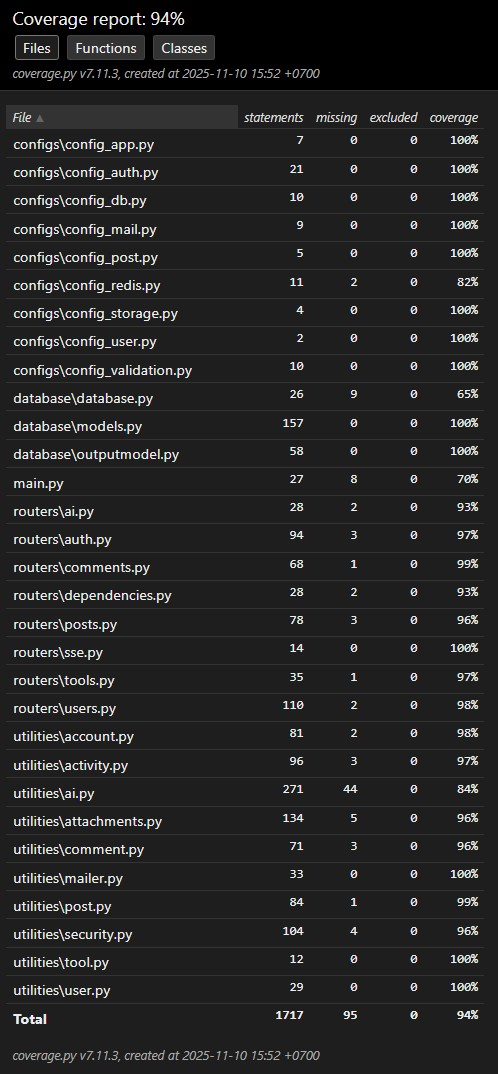
\includegraphics[width=0.5\textwidth]{backend_covjpg.jpg}
    \label{fig:backend_coverage}
\end{figure}

Ứng dụng phía máy chủ sử dụng thư viện pytest để thực hiện kiểm thử tự động, cùng với các thư viện bổ trợ để giả lập cơ sở dữ liệu hay bộ nhớ đệm và kiểm thử tích hợp API.
Thư viện này cho phép chạy các ca kiểm thử với các thiết lập tùy chỉnh, và hỗ trợ đo độ phủ của chương trình Python rất tốt, bao gồm báo cáo tổng quan khả năng bao phủ của kiểm thử, cũng như chỉ rõ những dòng lệnh nào đã được duyệt qua khi chạy kiểm thử.
Các kịch bản kiểm thử được viết bám sát với các ca sử dụng thực tế để giảm bớt số bài kiểm thử, nhưng vẫn đảm bảo kiểm tra được hết các chức năng nghiệp vụ và độ phủ mã lệnh cao nhất có thể.
Tại thời điểm kiểm thử ngày 10/11/2025, các ca kiểm thử đã phủ được tới 94\% mã nguồn hệ thống. Các phần không được kiểm tra chủ yếu đến từ việc xử lí ngoại lệ của các thư viện bên ngoài mà khó có thể tái tạo được trong ca kiểm thử.
Vào lần kiểm tra mới nhất sau khi cập nhật, sửa lỗi và tối ưu, độ phủ có chút giảm xuống còn 92\% do chưa có điều kiện viết thêm các ca kiểm thử mới.

\end{document}